\section{Purpose}
The  goal of the Requirement Analysis and Specification Document (RASD) is to give a clear description of the system that is going to be developed, its functional and non-functional requirements, its constraints and its domain. Moreover, it provides information about the relationship between the system taken into account and the external world by providing use cases and scenarios. Finally it gives a more formal specification of the most relevant features of the system to be using the Alloy language.
Generally this type of document is mainly addressed to developers, programmers, testers, project managers and system analysists, but it can be useful also for final users.
Track Me is a company that wants to develop three different but connected software-based services:
\begin{itemize}
  \item \textbf{Data4Help}: a service that allows third parties to monitor the location and health status of individuals. Through this service third parties can request the access both to the data of some specific individuals, who can accept or refuse sharing their information , and to anonymized data of group of individuals, which will be given only if the number of the members of the group is higher than 1000, according to privacy rules.
  \item \textbf{AutomatedSOS}: a service addressed to elderly people which monitors the health status of the subscribed customers and, when such parameters are below a certain threshold (personalized for every user using the data from Data4Help), sends to the location of the customer an ambulance, guaranteeing a reaction time less than 5 second from the time the parameters are below the threshold.
  % \clearpage
  \item \textbf{Track4Run}: a service to track athletes participating in a run. It allows organizers to define the path for a run, participants to enroll to a run and spectators to see on a map the position of all runners during the run. This service will exploit the features offered by Data4Help.
\end{itemize}

\subsection{Goals}
The three applications of the system have in common the following goals:
\begin{itemize}
  \item \textbf{[G.1]}: Allow unregistered user to sign in to access to the application;
  \item \textbf{[G.2]}: Allow registered user to log in and access to the application;
  \item \textbf{[G.3]}: Allow registered user to manage his/her profile;
\end{itemize}

The description given above can be summarized as a list of goals, specific for each service.
\paragraph{Data4Help:}
\begin{itemize}
  \item \textbf{[G.4]}: Allow registered third parties to request data of a single individual;
  \item \textbf{[G.5]}: Allow registered third parties to request data of a group of people;
\end{itemize}

\paragraph{AutomatedSOS:}
\begin{itemize}
  \item \textbf{[G.6]}: Allow data acquisition through smart watches (or similar);
  \item \textbf{[G.7]}: Allow monitoring the health status of an individual registered user;
  \item \textbf{[G.8]}: Allow sending location of an individual registered user to an ambulance if his/her parameters are below a certain threshold;
\end{itemize}

\paragraph{Track4Run:}
\begin{itemize}
  \item \textbf{[G.9]}: Allow registered user to become organizers or athletes of a run;
  \item \textbf{[G.10]}: Allow organizers to define the date and the path for a new run;
  \item \textbf{[G.11]}: Allow registered athletes to enroll to a run;
  \item \textbf{[G.12]}: Allow unregistered user to access as spectator;
  \item \textbf{[G.13]}: Allow registered/unregistered user to see on a map the position of all runners during a run;
\end{itemize}

\section{Scope}
According to \textit{The World and the Machine} \cite{world-machine} we can divide every system into two parts:
\begin{itemize}
  \item The \textbf{machine}, which is the portion of system to be developed;
  \item The \textbf{world}, which is the portion of the real-world affected by the machine.
\end{itemize}
As a consequence we can classify phenomena in three different types:
\begin{itemize}
  \item \textbf{World phenomena}: phenomena that the machine cannot observe;
  \item \textbf{Machine phenomena}: phenomena located entirely in the machine;
  \item \textbf{Shared phenomena}: phenomena that can be controlled by the world and observed by the machine or controlled by the machine and observed by the world;
\end{itemize}
Below we give an analysis of world and shared phenomena:
\paragraph{World phenomena}
\begin{itemize}
  \item A user turns on data connection;
  \item A user wears his smartwatch during a day;
  \item The batteries of the smartwatch of a user run out;
  \item A user turns on the GPS;
  \item An enrolled runner for a run takes part in it;
  \item A runner wears his smartwach during a run.
\end{itemize}
\paragraph{Shared phenomena}
\begin{itemize}
  \item New user registeres to Data4Help service;
  \item A Data4Help registered user logs into the system;
  \item A user recives a request to share his data;
  \item A user accept/decline a request to share his data;
  \item A third party requires data of a specific user;
  \item A third party requires data of a group of users;
  \item A user subscribes to AutomatedSOS service;
  \item An ambulance is called as a consequence of specific acquired data from the system;
  \item A Data4Help user access to Track4Run for the first time;
  \item A Track4Run user organizes a new run;
  \item A Track4Run user enrols for a run;
  \item An unregistered user access as a spectator to a run.
\end{itemize}
\paragraph{Machine phenomena}
\begin{itemize}
  \item The machine interfaces with external software and hardware systems;
  \item The machine manages database queries;
  \item The machine manages the 3G/4G Internet connection;
  \item The machine manages the Bluetooth connection;
  \item The machine manages GPS tracking.
\end{itemize}

\begin{figure}[H]
\begin{center}
  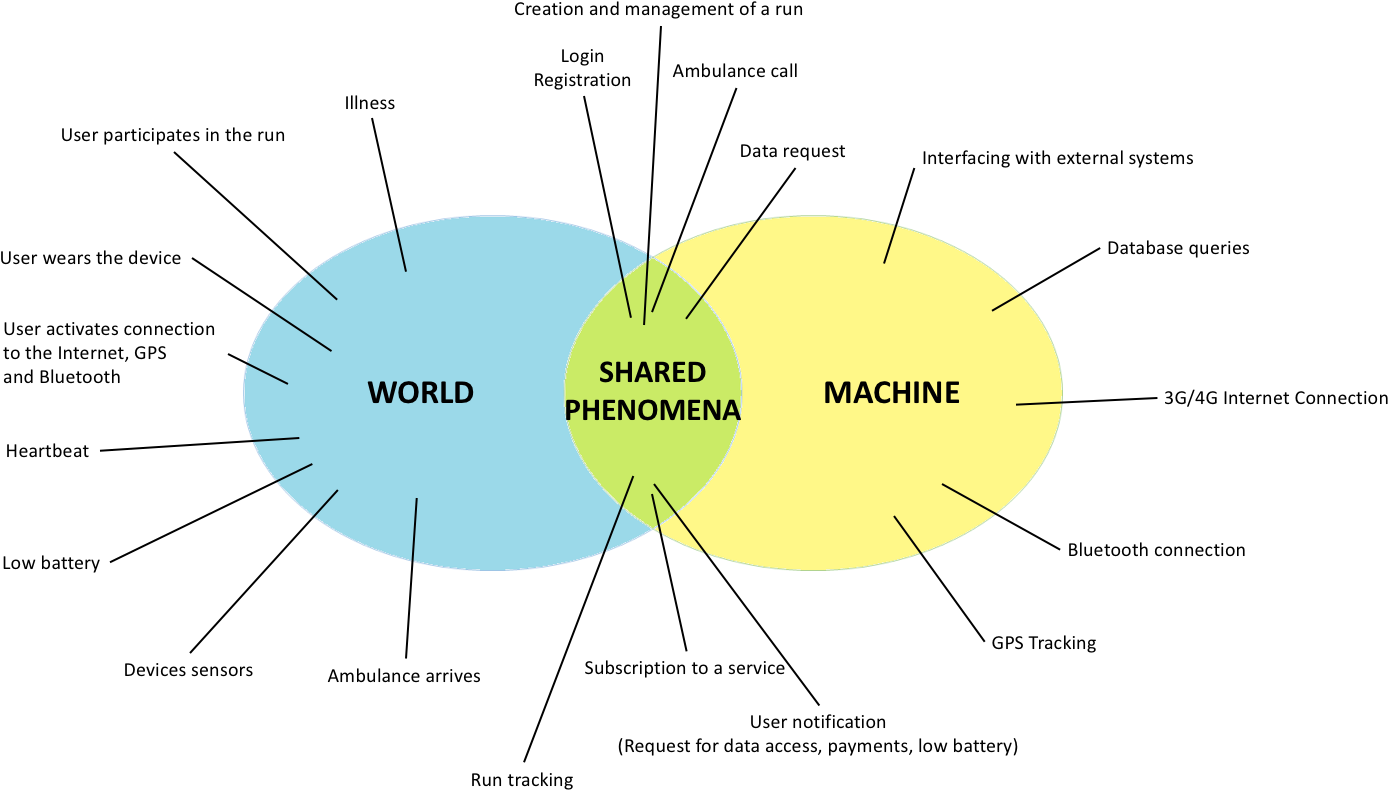
\includegraphics[width=\textwidth]{img/WorldMachine.png}
  \hspace{0.05\linewidth}
  \centering
  \caption{World and Machine model}
  \label{img:WandMmodel}
\end{center}
\end{figure}

\section{Definitions, Acronyms and Abbreviations}
\begin{itemize}
  \setlength{\itemindent}{-.4in}
  \item[] \textbf{API}: Application Programming Interface;
  \item[] \textbf{GPS}: Global Positioning System;
  \item[] \textbf{Organizer}: A registered user that organizes a run, defining date and path;
  \item[] \textbf{OS}: Operating System;
  \item[] \textbf{RASD}: Requirement Analysis and Specification Document;
  \item[] \textbf{Run}: An event that is organized by one organizer, at which one or more people can partecipate and that can be followed by one or more spectators;
  \item[] \textbf{Runner}: A registered user that enrols for a run;
  \item[] \textbf{Spectator}: Unregistered user that access to Track4Run to follow a run;
  \item[] \textbf{System}: The software system-to-be, including all of its services;
  \item[] \textbf{Third party}: Any external organization that wants to access to data acquired by Data4Help;
  \item[] \textbf{UML}: Unified Modeling Language;
  \item[] \textbf{User}: Any person, registered or not, who accesses to one of the applications (for Data4Help there is a special user called \textit{Third party});
  \item[] \textbf{VAT}: Value Added Tax.
\end{itemize}

\section{Reference documents}
------------------ TODO ------------------

\section{Overview}
This document is structured as follows:
\begin{itemize}
  \setlength{\itemindent}{-.4in}
  \item[] \textbf{Section 1: Introduction}. A general introduction to the goals, the phenomena and the scope of the system-to-be. It aims giving general but exaustive information about what this document is going explain.
  \item[] \textbf{Section 2: Overall Description}.
  \item[] \textbf{Section 3: Specific Requirements}.
  \item[] \textbf{Section 4: Effort Spent}. A summary of the worked time by each member of the group.
\end{itemize}
At the end there is the bibliography.
